
\centering
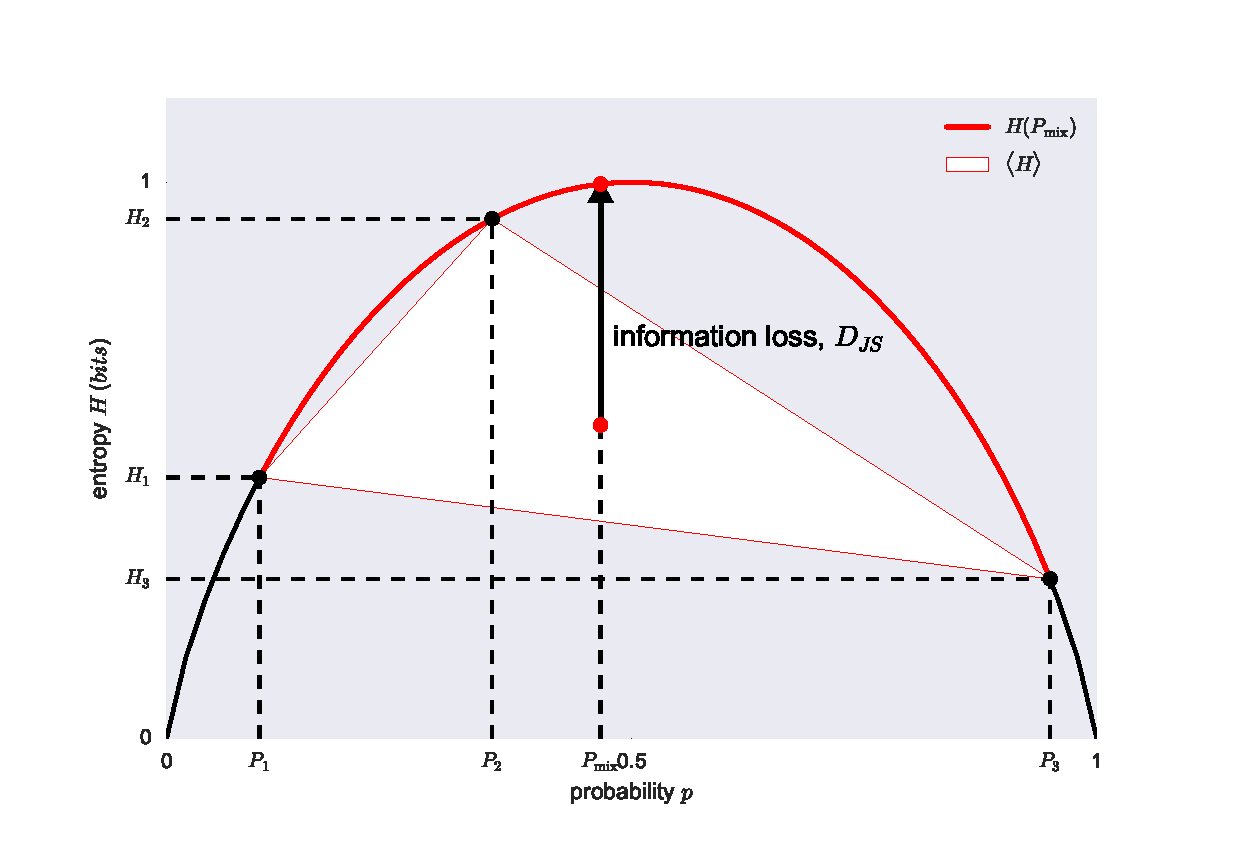
\includegraphics[width=1\textwidth]{jsd_entropy.eps}
\caption{
    Jensen-Shannon Divergence as mixing entropy.
    The graph shows the entropy $H$ of a discrete binary probability distribution function (PDF) $f(\{x_1, x_2\})$ as a function of the probability $p=f(x_1)=1-f(x_2)$.
    The black points show the location of three example PDFs, $f_1$, $f_2$ and $f_3$, in this space.
    Features highlighted in red are quantities entering the Jensen-Shannon Divergence (JSD).
    The entropy of the mixture $H(f_\text{mix})$ can lie anywhere on the red segment of the curve.
    The average entropy, $\langle H \rangle$, is restricted to the area designated by the triangle.
    }
\label{fig:jsd_entropy}

